%!TEX root = ../main.tex
%%%%%%%%%%%%%%%%%%%%%%%%%%%%%%%%%%
% Links:
%
% Difficulty:
% Companies: 
%%%%%%%%%%%%%%%%%%%%%%%%%%%%%%%%%%

\chapter{$n^{th}$ node from the end}
\label{ch:node_from_the_end}
\section*{Introduction}
The problem presented in this chapter is a particularly interesting one on Linked List. It has been asked numerous times in companies like Amazon and Google and it is therefore important that we understand and master the solution to this problem.

\section{Problem statement}
\begin{exercise}
Given a linked list $L$ (which definition is shown in Listing \ref{list:delete_duplicates_list:linked_list} at page \pageref{list:delete_duplicates_list:linked_list} , and an integer $n$ remove the $n^{th}$ node from the end of list.

\begin{example}
	\hfill \\
	Given $L=[1,2,3,4]$, and $n=2$ the function returns: $L=[1,2,4]$. See Figure \ref{fig:node_from_the_end:example1}.
\end{example}

\begin{example}
	Given $L=[1,2,3,4]$, and $n=0$ the function returns: $L=[1,2,4]$.
	See Figure \ref{fig:node_from_the_end:example2}.
\end{example}
\end{exercise}


\begin{figure}
	\label{fig:node_from_the_end:example1}
	\centering
	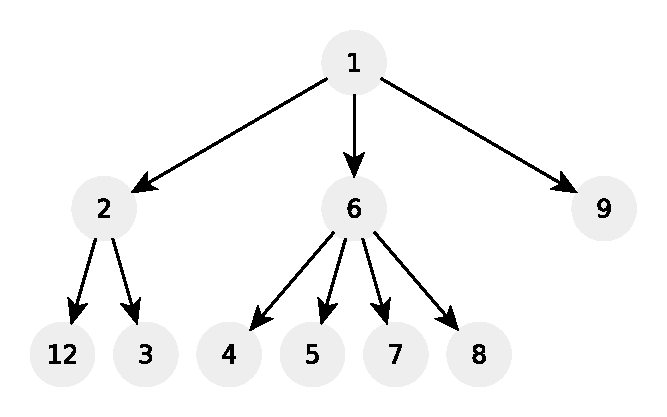
\includegraphics[scale=1.0]{sources/node_from_the_end/images/example1}
	\caption{Removal of the \nth{2} to last element in a singly linked list of length $4$.}
\end{figure}

\begin{figure}
	\label{fig:node_from_the_end:example2}
	\centering
	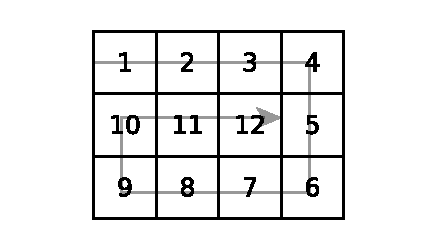
\includegraphics[scale=1.0]{sources/node_from_the_end/images/example2}
	\caption{Removal of the \nth{4} to last element in a singly linked list of length $4$. The head pointer needs to be updated.}
\end{figure}


\section{Clarification Questions}

\begin{QandA}
	\item Is $n$ guaranteed to be a valid node in the list?
	\begin{answered}
		\textit{Yes you can assume that $n$ is the index of a valid node in the list.}
	\end{answered}
\end{QandA}

\section{Discussion}
\label{node_from_the_end:sec:discussion}
This problem has two main parts in it: 
\begin{enumerate}
	\item Finding out the index of the $n$-to last node
	\item Removing a node from the list
\end{enumerate}
Those tasks are separate and thus we can solve each of them separately and then use the solution to these two subproblems to obtain our final answer.

\subsection{Brute-force}
\label{node_from_the_end:sec:bruteforce}
Finding out the the node to be deleted becomes trivial once we know how long the list is. Therefore the brute-force approach simply performs a first pass in the list and counts how many nodes it is made of i.e. $l$. Then it performs another pass but it stops at node $l-n$ (the n-to-last node) and removes it.
Please note that in order to correctly remove a node from a singly linked list a we need to have a pointer to the node we want to remove as well as a pointer to its predecessor (variable \inline{pred} in the code). This approach can be implemented as shown in Listing \ref{list:node_from_the_end:bruteforce}, and it has a time and space complexity of  $O(n)$ and $O(1)$, respectively.


\lstinputlisting[language=c++, caption={Sample Caption},label=list:node_from_the_end:bruteforce]{sources/node_from_the_end/node_from_the_end_solution1.cpp}



\subsection{Common Variation}
\subsubsection{List midpoint}
\label{node_from_the_end:sec:list_midpoint}
